\documentclass[12pt]{article}
\usepackage{graphicx}
\usepackage{float}
\usepackage{amsmath}
\begin{document}
\title{Statistics 12, Lab 4}
\date{March 5th, 2019}
\author{Michael Wu\\UID: 404751542}
\maketitle

\section*{Exercise 1}

\paragraph{a)}

I ran the following code.
\begin{verbatim}
head(pawnee)
dim(pawnee)
\end{verbatim}
This output the following data.
\begin{verbatim}
  ï..ID Latitude Longitude Arsenic Sulfur New_hlth_issue
1     1 41.09414 -85.60974       0      0              N
2     2 41.09054 -85.70344       0    130              N
3     3 41.08601 -85.71996       4    170              N
4     4 41.08100 -85.75415       0      0              Y
5     5 41.07435 -85.70043       0      0              N
6     6 41.07399 -85.71788       0      0              N
\end{verbatim}
It also output that there are 541 rows and 6 columns.

\paragraph{b)}

I ran the following code.
\begin{verbatim}
set.seed(1337)
pawneeSample <- pawnee[sample(nrow(pawnee), size=30),]
head(pawneeSample)
\end{verbatim}
This output the following data.
\begin{verbatim}
    ï..ID Latitude Longitude Arsenic Sulfur New_hlth_issue
312   312 41.01716 -85.66949     1.0      0              N
305   305 41.01742 -85.65858     0.5     40              N
40     40 41.06414 -85.72544     0.0      0              N
245   245 41.02714 -85.73328     0.0      0              N
201   201 41.03244 -85.63653     0.0      0              N
178   178 41.03568 -85.64353     0.0      0              Y
\end{verbatim}

\paragraph{c)}

I ran the following code.
\begin{verbatim}
mean(pawneeSample$Arsenic)
mean(pawneeSample$New_hlth_issue=="Y")
\end{verbatim}
This output the sample mean arsenic level of 5.566667 parts per million. The sample proportion of
households experiencing a major health issue is 26.66667\%.

\paragraph{d)}

We would use the symbol \(\bar{x}\) for the mean arsenic level since it is a sample mean. We would use
the symbol \(\hat{p}\) for the proportion of health issues since it is a sample proportion.

\paragraph{e)}

The confidence levels of 90\%, 95\%, and 99\% have critical values of 1.645, 1.96, and 2.576, respectively.
We will calculate the standard deviation using the sample proportion as follows.
\[\sqrt{\frac{0.2666667\times0.7333333}{30}}=0.0807\]
Then the confidence intervals for these confidence levels are the following.
\begin{align*}
    0.2666667\pm1.645\times0.0807&=(0.1335117,0.3998217)\\
    0.2666667\pm1.96\times0.0807&=(0.1084947,0.4248387)\\
    0.2666667\pm2.576\times0.0807&=(0.0587835,0.4745499)
\end{align*}

\paragraph{f)}

The bounds of a 100\% confidence interval for the population proportion would be between
0\% and 100\%. This is the range of all possible values that the proportion will be, so we
know the proportion will be in this range.

\paragraph{g)}

I ran the following code.
\begin{verbatim}
mean(pawnee$New_hlth_issue=="Y")
\end{verbatim}
This output that the true proportion of houses experiencing a new health issue is 29.20518\%.

\paragraph{h)}

I ran the following code.
\begin{verbatim}
histogram(pawnee$Arsenic, main="Arsenic Levels in Pawnee",
          xlab="Arsenic (ppm)", ylab="Homes", type="count")
\end{verbatim}
This generated the following plot.
\begin{figure}[H]
    \begin{center}
        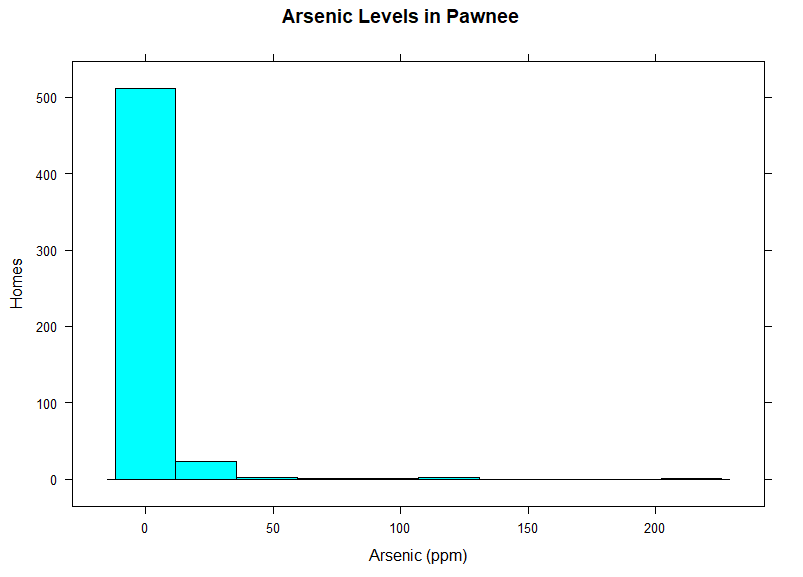
\includegraphics[width=4.5in]{exercise1h.png}
    \end{center}
\end{figure}

\section*{Exercise 2}

\paragraph{a)}

I ran the following code.
\scriptsize
\begin{verbatim}
n <- 30
N <- 541
M <- 1000
phats <- c()
set.seed(123)
for(i in 1:M){
  index <- sample(N, size = n)
  sample_i <- pawnee[index,]
  phats[i] <- mean(sample_i$New_hlth_issue == "Y")
}
histogram(phats, main="Sampling Distribution of Health Issue Proportions in Pawnee",
          xlab="Sample Health Issue Proportion", type="density", density=TRUE,
          fit="normal")
\end{verbatim}
\normalsize
This generated the following plot.
\begin{figure}[H]
    \begin{center}
        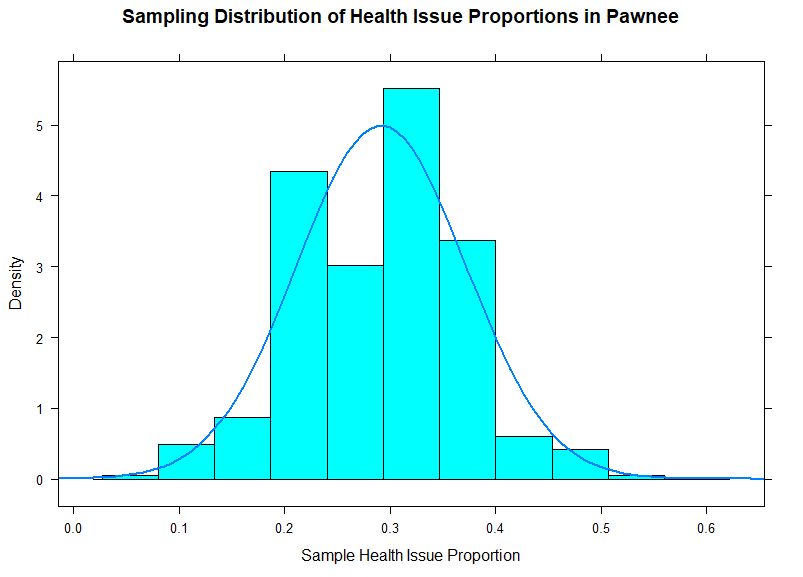
\includegraphics[width=4.5in]{exercise2a.png}
    \end{center}
\end{figure}

\paragraph{b)}

I ran the following code.
\begin{verbatim}
mean(phats)
sd(phats)
\end{verbatim}
This output that the mean of the simulated sample proportions was 0.2914333
and the standard deviation was 0.07997713.

\paragraph{c)}

Yes I believe the simulated distribution of sample proportions is approximately
normal. This is because the normal curve that was superimposed on the previous
histogram fits the actual data fairly well. Additionally, we have run a large
number of simulations with a large enough sample size such that the Central
Limit Theorem comes into effect.

\paragraph{d)}

In theory the mean of the sampling distribution of sample proportions should be the
same as the true population proportion 0.2920518. The standard deviation should
be the following value.
\[\sqrt{\frac{0.2920518\times0.7079482}{30}}=0.08301758\]
The experimental values I obtained matched these theoretical values fairly well.
The experimental mean proportion was only 0.0006185 below the theoretical mean proportion.
The experimental standard deviation was only 0.00304045 below the theoretical standard
deviation.

\section*{Exercise 3}

\paragraph{a)}

I ran the following code.
\begin{verbatim}
n <- 30
N <- 541
M <- 1000
phats <- c()
set.seed(123)
for(i in 1:M){
  index <- sample(N, size = n)
  sample_i <- pawnee[index,]
  phats[i] <- mean(sample_i$Arsenic)
}
\end{verbatim}

\paragraph{b)}

I ran the following code.
\scriptsize
\begin{verbatim}
histogram(phats, main="Sampling Distribution of Arsenic Levels in Pawnee",
          xlab="Sample Mean Arsenic (ppm)", type="density", density=TRUE,
          fit="normal")
\end{verbatim}
\normalsize
This generated the following plot.
\begin{figure}[H]
    \begin{center}
        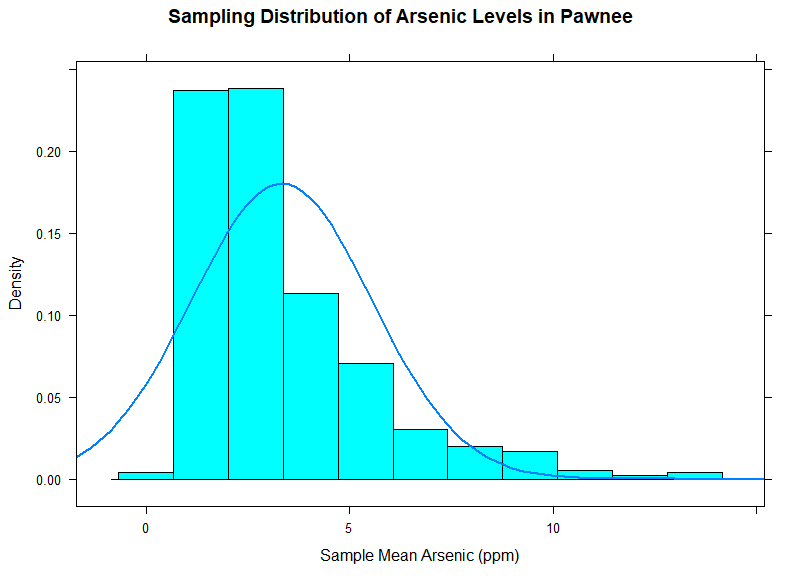
\includegraphics[width=4.5in]{exercise3a.png}
    \end{center}
\end{figure}

\paragraph{c)}

I do not think the simulated distribution of arsenic means is approximately normal.
Clearly this distribution is skewed right. This conclusion differs from my previous
conclusion that the distribution of sampling proportions is approximately normal because
the input distribution of arsenic is heavily skewed right. So we would need to increase
the sample size in order to counteract the skew of the input distribution.

\end{document}